\documentclass[xcolor=table]{beamer}

\usepackage{lscape, amsmath, amsfonts, amssymb, setspace, theorem, wrapfig, graphicx, float, multirow, subfig, color, rotating, multicol, datetime, natbib, venndiagram, pstricks, xkeyval, tikz, etoolbox, verbatim, subfig}

\usepackage[super]{nth}
\usepackage{listings}
\usepackage{xcolor}
\usepackage{natbib}
\usepackage{tikz-cd}

\definecolor{codegreen}{rgb}{0,0.6,0}
\definecolor{codegreengray}{rgb}{0,0.4,0}
\definecolor{codegray}{rgb}{0.5,0.5,0.5}
\definecolor{codeblue}{rgb}{0.00,0,0.82}
\definecolor{backcolour}{rgb}{0.95,0.95,0.92}
 
\lstdefinestyle{mystyle}{
    backgroundcolor=\color{backcolour},   
    commentstyle=\color{codegreengray},
    numberstyle=\tiny\color{codegray},
    stringstyle=\color{codegreen},    basicstyle=\ttfamily\footnotesize,
    breakatwhitespace=false,         
    breaklines=true,                 
    captionpos=b,                    
    keepspaces=true,                 
    numbers=left,                    
    numbersep=5pt,                  
    showspaces=false,                
    showstringspaces=false,
    showtabs=false,                  
    tabsize=2
}
 
\lstset{style=mystyle}

\title{GV300 - Quantitative Political Analysis}
\subtitle{University of Essex - Department of Government}
\date{Week 16 -- 13 January, 2020}				% or you can specify a date, just write it down instead of "\today"
\author{Lorenzo Crippa} 

\usetheme[progressbar=frametitle]{metropolis}
\usecolortheme{seahorse}						% try others: wolverine; crane...

\begin{document}

\frame{
\titlepage
}

\frame{
\frametitle{Communication}
\begin{center}
For the spring term, new office hour:

Monday 14:00 to 16:00 (before class) \\ Office 5B.153
\end{center}
}

\frame{
\frametitle{Midterm exam -- Question 4 (a)}
Create a 1000 observation dataset. Generate variables RootCause and OtherThing as independent, uncorrelated variables each drawn from a normal distribution with mean 0 and variance 1.

Create a set of normal error terms with mean 0 and variance 1. Let $Outcome = 1 + RootCause + 3*OtherThing + errors$.
}

\begin{frame}[fragile]
\frametitle{Question 4 -- (a) i.}
Draw a graphical representation of the data generating process (DGP) involving
the variables Outcome, RootCause, and OtherThing. \pause Are RootCause and
OtherThing independent? \pause How would you represent graphically that they are independent in your DGP? \pause

\begin{center}
\begin{tikzcd}
RootCause \arrow[rrrd] &  &  &         \\
OtherThing \arrow[rrr] &  &  & Outcome
\end{tikzcd}
\end{center}
\end{frame}

\begin{frame}
\frametitle{Question 4 -- (a) ii. and iii.}
Regress Outcome on RootCause. Report and interpret the result. \pause Did you
estimate the causal effect of RootCause on Outcome with this regression? Why? \pause

Regress Outcome on RootCause and OtherThing. Report and interpret the result. \pause Did you estimate the causal effect of RootCause on Outcome? Why?
\end{frame}

\begin{frame}
\frametitle{Question 4 -- (a) ii. and iii. results}
\begin{table}[!htbp] 
\centering 
\resizebox{80mm}{38mm}{
\begin{tabular}{@{\extracolsep{5pt}}lcc} 
\\[-1.8ex]\hline 
\hline \\[-1.8ex] 
 & \multicolumn{2}{c}{\textit{Dependent variable:}} \\ 
\cline{2-3} 
\\[-1.8ex] & \multicolumn{2}{c}{Outcome} \\ 
\\[-1.8ex] & (ii.) & (iii.)\\ 
\hline \\[-1.8ex] 
 RootCause & 0.860$^{***}$ & 0.998$^{***}$ \\ 
  & (0.102) & (0.033) \\ 
  & & \\ 
 OtherThing &  & 3.023$^{***}$ \\ 
  &  & (0.033) \\ 
  & & \\ 
 Constant & 1.079$^{***}$ & 1.053$^{***}$ \\ 
  & (0.101) & (0.033) \\ 
  & & \\ 
\hline \\[-1.8ex] 
Observations & 1,000 & 1,000 \\ 
R$^{2}$ & 0.067 & 0.901 \\ 
Adjusted R$^{2}$ & 0.066 & 0.901 \\ 
F Statistic & 71.340$^{***}$ (df = 1; 998) & 4,528.766$^{***}$ (df = 2; 997) \\ 
\hline 
\hline \\[-1.8ex] 
\textit{Note:}  & \multicolumn{2}{r}{$^{*}$p$<$0.1; $^{**}$p$<$0.05; $^{***}$p$<$0.01} \\ 
\end{tabular} 
}
\end{table} 
\end{frame}

\begin{frame}
\frametitle{Question 4 -- (a) ii. and iii. causal effects}
\begin{itemize}
\item Remember the ``true'' values of the parameters associated with RootCause and OtherThing are $+1$ and $+3$ respectively. ``True'' constant term is $+1$ \pause

\item In both models ii. and iii. we estimate the causal effect of RootCause on Outcome, because in none of these cases there is a confounder involved in the DGP. \pause 

\item OtherThing is not a confounder in model ii.: it does not generate an OVB issue. \pause The zero conditional mean assumption is met in both cases.
\end{itemize}
\end{frame}

\begin{frame}
\frametitle{Question 4 -- (a) iv.}
Compare the results of the regressions you ran in 4a.ii and 4a.iii. \pause

\begin{itemize}
\item Model iii. is more precise in its estimate of the causal effect of RootCause, because it models explicitly one factor of the DGP of Outcome (OtherThing), which remains in the error term for model ii. \pause

\item Therefore the estimate of the parameter associated with RootCause is closer to the ``true'' value in model iii. \pause

\item For the same reason model iii. also performs better in terms of $R^2$ and $F$ statistics: it explains more variance of the dependent variable.
\end{itemize}
\end{frame}

\frame{
\frametitle{Midterm exam -- Question 4 (b)}
Create a 1000 observation dataset. Generate variable RootCause following a normal distribution with mean 0 and variance 1. Generate variable $OtherThing = 2*RootCause + noise$ where noise follows a normal distribution with mean 0 and
variance 1. 

Create a set of normal error terms with mean 0 and variance 1. Let $Outcome = 1
+ RootCause + 3*OtherThing + errors$.
}

\begin{frame}[fragile]
\frametitle{Question 4 -- (b) i.}
Draw a graphical representation of the data generating process (DGP) involving
the variables Outcome, RootCause, and OtherThing. \pause Are RootCause and
OtherThing independent? \pause

\begin{center}
\begin{tikzcd}
RootCause \arrow[rrrd] \arrow[d] &  &  &         \\
OtherThing \arrow[rrr]           &  &  & Outcome
\end{tikzcd}
\end{center}
\end{frame}

\begin{frame}
\frametitle{Question 4 -- (b) ii. and iii.}
Regress Outcome on RootCause. Report and interpret the result. \pause Did you
estimate the causal effect of RootCause on Outcome with this regression? Why? \pause

Regress Outcome on RootCause and OtherThing. Report and interpret the result. \pause Did you estimate the causal effect of RootCause on Outcome? Why?
\end{frame}

\begin{frame}
\frametitle{Question 4 -- (b) ii. and iii. results}
\begin{table}[!htbp] 
\centering 
\resizebox{80mm}{38mm}{
\begin{tabular}{@{\extracolsep{5pt}}lcc} 
\\[-1.8ex]\hline 
\hline \\[-1.8ex] 
 & \multicolumn{2}{c}{\textit{Dependent variable:}} \\ 
\cline{2-3} 
\\[-1.8ex] & \multicolumn{2}{c}{Outcome} \\ 
\\[-1.8ex] & (ii.) & (iii.)\\ 
\hline \\[-1.8ex] 
 RootCause & 6.893$^{***}$ & 0.994$^{***}$ \\ 
  & (0.102) & (0.069) \\ 
  & & \\ 
 OtherThing &  & 3.003$^{***}$ \\ 
  &  & (0.031) \\ 
  & & \\ 
 Constant & 0.921$^{***}$ & 1.009$^{***}$ \\ 
  & (0.100) & (0.031) \\ 
  & & \\ 
\hline \\[-1.8ex] 
Observations & 1,000 & 1,000 \\ 
R$^{2}$ & 0.820 & 0.982 \\ 
Adjusted R$^{2}$ & 0.820 & 0.982 \\ 
F Statistic & 4,540.510$^{***}$ (df = 1; 998) & 27,733.450$^{***}$ (df = 2; 997) \\ 
\hline 
\hline \\[-1.8ex] 
\textit{Note:}  & \multicolumn{2}{r}{$^{*}$p$<$0.1; $^{**}$p$<$0.05; $^{***}$p$<$0.01} \\ 
\end{tabular} 
}
\end{table} 
\end{frame}

\begin{frame}
\frametitle{Question 4 -- (b) ii. and iii. causal effects}
\begin{itemize}
\item Now only model iii. estimates the unbiased causal effect of RootCause on Outcome. In model ii., indeed, the zero conditional mean assumption is not met, because OtherThing is a confounder which is not explicitly modelled. \pause

\item In model ii., $E(errors|RootCause)\neq 0$ because something which is ``left'' in the error term (that is, OtherThing, which is not modelled) is caused by RootCause. \pause

\item Omitting OtherThing in model ii. generates an OVB issue, because the variable is a confounder in the DGP.
\end{itemize}
\end{frame}

\begin{frame}
\frametitle{Question 4 -- (b) iv.}
Compare the results of the regressions you ran in 4b.ii and 4b.iii.  \pause

\begin{itemize}
\item Model iii. is correct in its estimate of the causal effect of RootCause (and OtherThing), because it models explicitly all confounders of the DGP of Outcome. \pause Therefore its estimates of the parameters are unbiased. \pause

\item Model ii. obtains a biased estimate of the causal effect of RootCause on Outcome. \pause It is larger in absolute value, which makes sense because RootCause enters twice in the DGP of Outcome: directly and indirectly through OtherThing (see causal diagram, point 4b.i) \pause.

\item Notice that the bias of model ii. cannot be inferred by simply looking at statistics such as the $R^2$ and $F$ statistics.
\end{itemize}
\end{frame}

\begin{frame}[fragile]
\frametitle{Question 5 -- (a)}
Load the data set ``\texttt{gb\_recoded.dta}''. Provide appropriate summary statistics and plots for the variables \texttt{e5}, \texttt{age}, and
\texttt{turnout05}. \pause

Summary statistics in \texttt{R} (from package \texttt{psych}):
\begin{lstlisting}[language = R]
describe(data.frame(data$age, data$gender, data$f1, data$e5, data$turnout05))
\end{lstlisting} \pause

Summary statistics in Stata:
\begin{lstlisting}
summarize age gender f1 e5 turnout05 
\end{lstlisting}
\end{frame}

\begin{frame}[fragile]
\frametitle{Question 5 -- (a)}
Summary statistics output (from \texttt{R}):
\begin{lstlisting}
                  n  mean    sd min max range   se
data.age       2301 47.01 15.21  18  88    70 0.32
data.gender*   1732  1.51  0.50   1   2     1 0.01
data.f1*       2301  3.70  3.00   1   9     8 0.06
data.e5*       2300  2.72  1.49   1   7     6 0.03
data.turnout05 2301  0.81  0.39   0   1     1 0.01
\end{lstlisting} \pause

\texttt{*}: these variables are factors. \texttt{R} recognizes them as such.
\end{frame}

\begin{frame}[fragile]
\frametitle{Question 5 -- (a)}
Plots in \texttt{R} (from package \texttt{ggplot2}): \pause
\begin{lstlisting}[language = R]
# e5
ggplot(data, aes(x = e5)) + geom_bar() 

# age
ggplot(data, aes(x = age)) + geom_density()

# turnout05
ggplot(data, aes(x = turnout05)) + 
	geom_bar(stat = "count")
	
# multivariate
ggplot(data, aes(y = age, x = f1)) + geom_boxplot() + 
  theme(axis.text.x = element_text(angle = 15))
\end{lstlisting}
\end{frame}

\begin{frame}[fragile]
\frametitle{Question 5 -- (a)}
Plots in Stata: \pause
\begin{lstlisting}
* e5
hist e5, discrete xtitle("opinion") xlabel(, valuelabel)

* age
kdensity age

* turnout05
hist turnout05, discrete xlabel(0 1) xtitle("turnout 2005")
	
* multivariate
graph box age, over(f1)
\end{lstlisting}
\end{frame}

\frame{
\frametitle{Question 5 -- (a)}
Variable \texttt{e5} (opinion), barplot
\begin{figure}
\centering
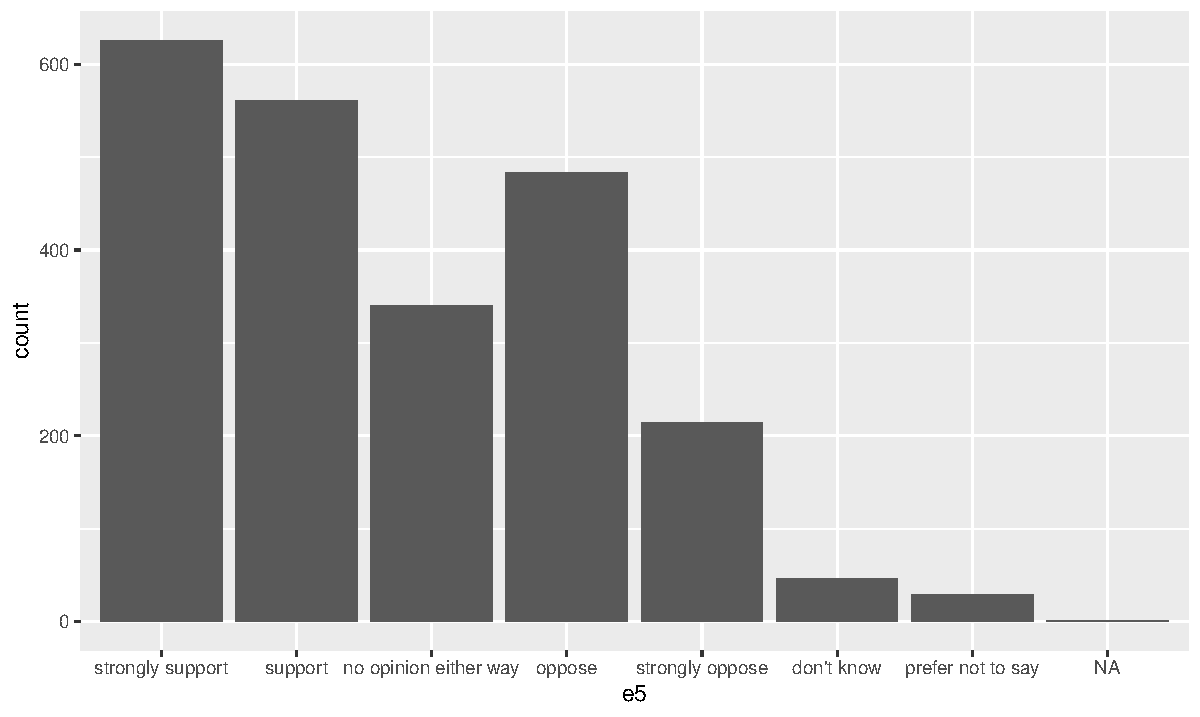
\includegraphics[width=110mm]{pictures/week_16_barplot.pdf}
\end{figure}
}

\frame{
\frametitle{Question 5 -- (a)}
Variable \texttt{age}, density
\begin{figure}
\centering
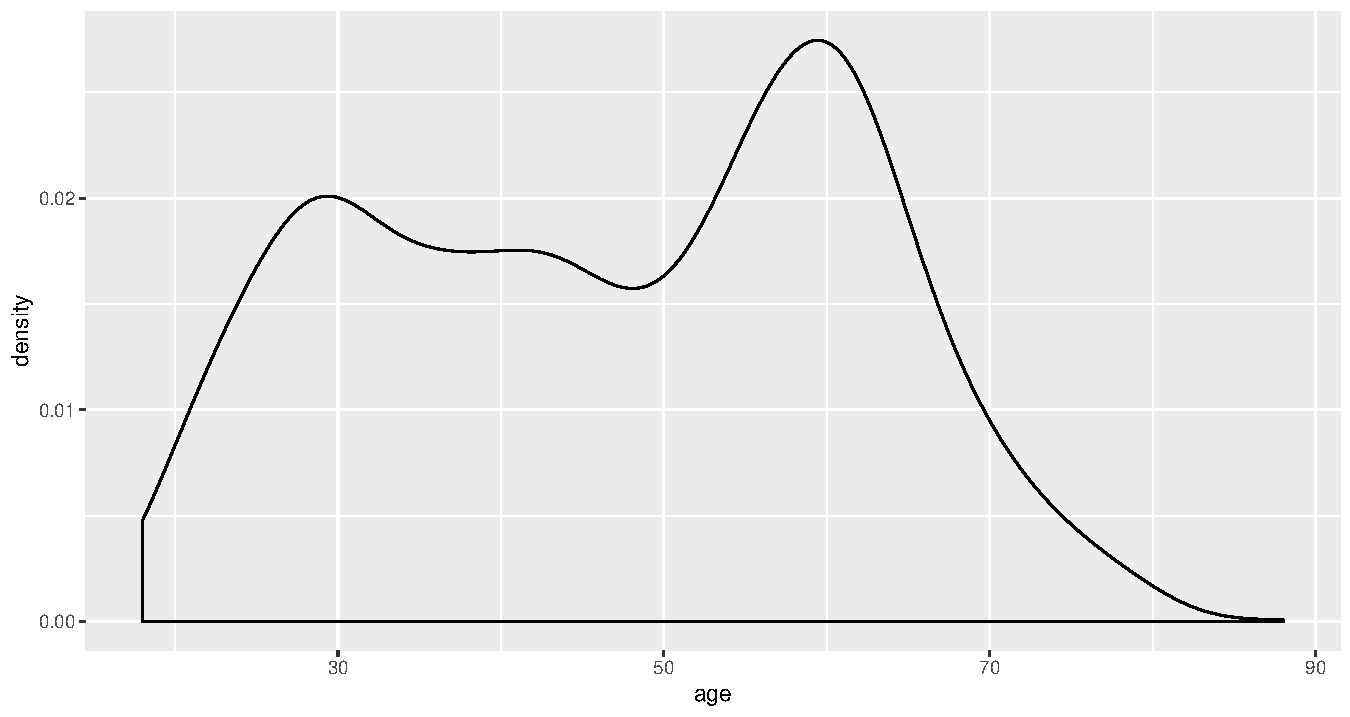
\includegraphics[width=110mm]{pictures/week_16_density.pdf}
\end{figure}
}

\frame{
\frametitle{Question 5 -- (a)}
Variable \texttt{turnout05} (2005 elections turnout), barplot
\begin{figure}
\centering
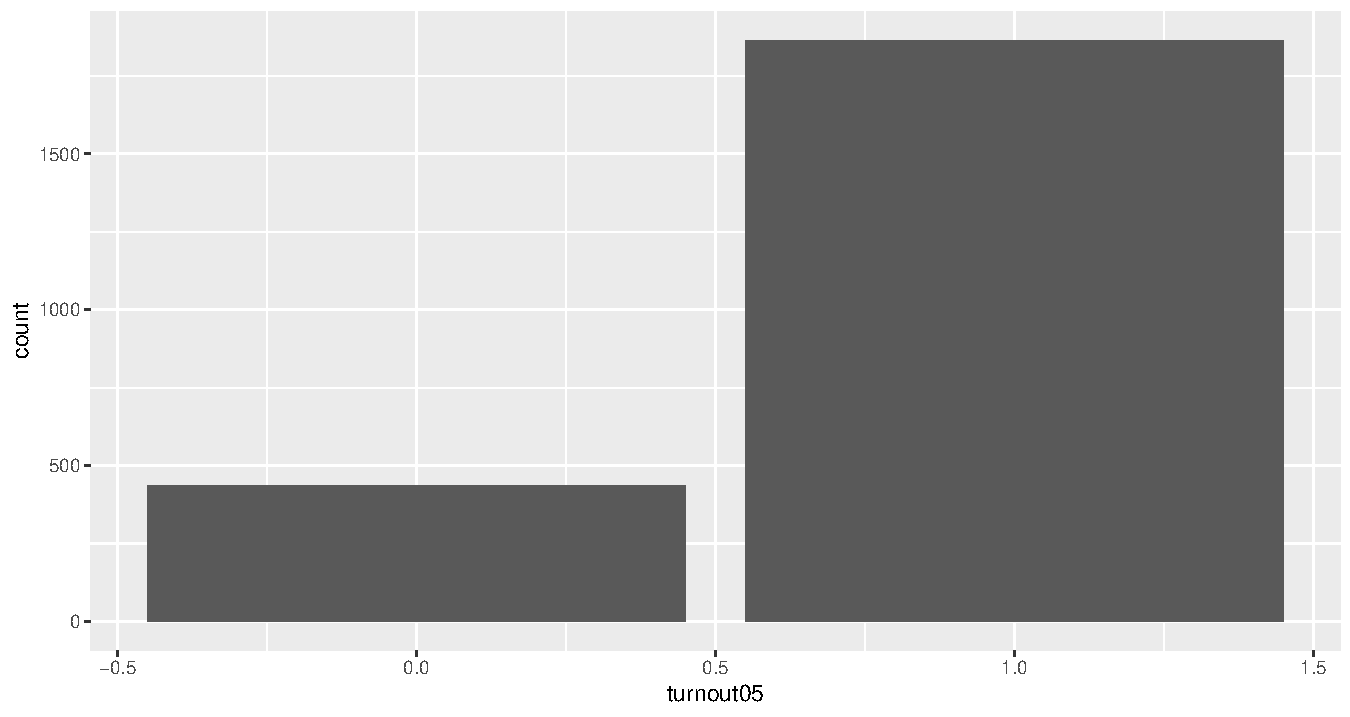
\includegraphics[width=110mm]{pictures/week_16_barplot2.pdf}
\end{figure}
}

\frame{
\frametitle{Question 5 -- (a)}
Variable \texttt{age} by \texttt{f1} (partisanship), boxplot
\begin{figure}
\centering
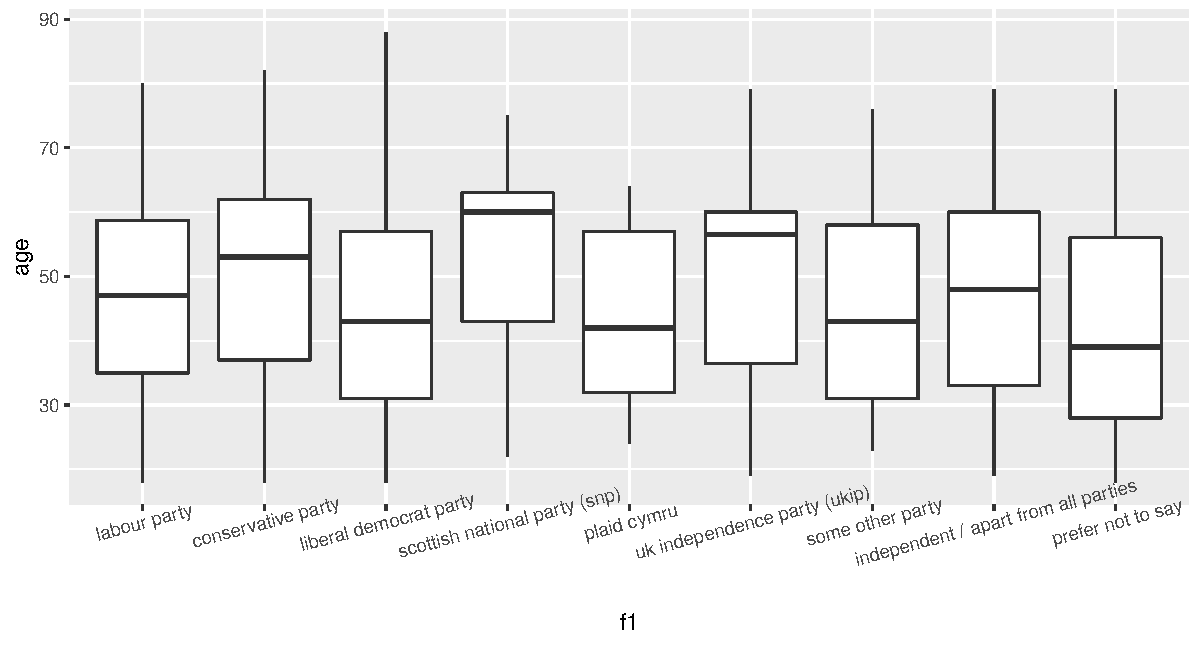
\includegraphics[width=110mm]{pictures/week_16_bivariate.pdf}
\end{figure}
}

\begin{frame}[fragile]
\frametitle{Question 5 -- (b)}
Create a reasonable model of public opinion as a function of the variables given above. Run a linear regression and interpret the outcome of that regression. \pause

Model:
\begin{center}
\begin{tikzcd}
gender \arrow[rrrd] \arrow[d] &  &  &         \\
partisanship \arrow[rrr] &  &  & opinion \\
age \arrow[rrru] \arrow[u] &  &  &        
\end{tikzcd}
\end{center} \pause

I argue turnout in 2005 elections is not part of the DGP of \textit{opinion}. It does not enter this causal model. \pause Note the confounding variables \textit{age} and \textit{gender}. We \textit{must} model them!
\end{frame}

\begin{frame}[fragile]
\frametitle{Question 5 -- (b)}
We have factor variables. \texttt{R} treats them automatically as factors. Tell the program to treat them as numeric if you want to. \pause

Model in \texttt{R}:
\begin{lstlisting}[language = R]
data$e5_num <- as.numeric(data$e5)
data$gender_num <- as.numeric(data$gender)
data$f1_num <- as.numeric(data$f1)

# only the dep. variable as non-factor
model.f <- lm(e5_num ~ age + gender + f1, data = data)

# all factor variables turned into non-factors
model.n <-lm(e5_num ~ age + gender_num + f1_num, 
	data = data)
	
# table
stargazer(model.f, model.n, type = "text")
\end{lstlisting}
\end{frame}

\begin{frame}[fragile]
\frametitle{Question 5 -- (b)}
Stata automatically treat factor variables as numeric. You need to tell the program to treat them as factors if you want to. \pause

Model in Stata:
\begin{lstlisting}
* only the dep. variable as non-factor
reg e5 age i.gender i.f1
est store model_f

* all factor variables turned into non-factors
reg e5 age gender f1
est store model_n

* table
esttab model_f model_n, scalars(N r2 r2_a F p) star(* .1 ** .05 *** .01)
\end{lstlisting}
\end{frame}

\begin{frame}
\frametitle{Question 5 -- (b)}
\begin{table}[!htbp] 
\centering 
\resizebox{45mm}{38mm}{
\begin{tabular}{@{\extracolsep{5pt}}lcc} 
\\[-1.8ex]\hline 
\hline \\[-1.8ex] 
 & \multicolumn{2}{c}{\textit{Dependent variable:}} \\ 
\cline{2-3} 
\\[-1.8ex] & \multicolumn{2}{c}{e5\_num} \\ 
\\[-1.8ex] & (1) & (2)\\ 
\hline \\[-1.8ex] 
 age & $-$0.019$^{***}$ & $-$0.020$^{***}$ \\ 
  & (0.002) & (0.002) \\ 
  & & \\ 
 genderfemale & $-$0.225$^{***}$ &  \\ 
  & (0.069) &  \\ 
  & & \\ 
 f1conservative party & $-$0.109 &  \\ 
  & (0.091) &  \\ 
  & & \\ 
 f1liberal democrat party & 0.184 &  \\ 
  & (0.129) &  \\ 
  & & \\ 
 f1scottish national party (snp) & 0.256 &  \\ 
  & (0.254) &  \\ 
  & & \\ 
 f1plaid cymru & $-$0.193 &  \\ 
  & (0.544) &  \\ 
  & & \\ 
 f1uk independence party (ukip) & $-$0.004 &  \\ 
  & (0.218) &  \\ 
  & & \\ 
 f1some other party & $-$0.117 &  \\ 
  & (0.208) &  \\ 
  & & \\ 
 f1independent / apart from all parties & 0.038 &  \\ 
  & (0.107) &  \\ 
  & & \\ 
 f1prefer not to say & 0.373$^{***}$ &  \\ 
  & (0.134) &  \\ 
  & & \\ 
 gender\_num &  & $-$0.228$^{***}$ \\ 
  &  & (0.069) \\ 
  & & \\ 
 f1\_num &  & 0.025$^{**}$ \\ 
  &  & (0.012) \\ 
  & & \\ 
 Constant & 3.731$^{***}$ & 3.931$^{***}$ \\ 
  & (0.139) & (0.171) \\ 
  & & \\ 
\hline \\[-1.8ex] 
Observations & 1,731 & 1,731 \\ 
R$^{2}$ & 0.055 & 0.048 \\ 
Adjusted R$^{2}$ & 0.049 & 0.047 \\ 
F Statistic & 9.990$^{***}$ (df = 10; 1720) & 29.217$^{***}$ (df = 3; 1727) \\ 
\hline 
\hline \\[-1.8ex] 
\textit{Note:}  & \multicolumn{2}{r}{$^{*}$p$<$0.1; $^{**}$p$<$0.05; $^{***}$p$<$0.01} \\ 
\end{tabular}
}
\end{table}
\end{frame}

\begin{frame}
\frametitle{Question 5 -- (b)}
\begin{table}[!htbp] 
\centering 
\resizebox{45mm}{38mm}{
\begin{tabular}{@{\extracolsep{5pt}}lc} 
\\[-1.8ex]\hline 
\hline \\[-1.8ex] 
 & \multicolumn{1}{c}{\textit{Dependent variable:}} \\ 
\cline{2-2} 
\\[-1.8ex] & e5\_num \\ 
\hline \\[-1.8ex] 
 age & $-$0.020$^{***}$ \\ 
  & (0.002) \\ 
  & \\ 
 gender\_num & $-$0.228$^{***}$ \\ 
  & (0.069) \\ 
  & \\ 
 f1\_num & 0.025$^{**}$ \\ 
  & (0.012) \\ 
  & \\ 
 Constant & 3.931$^{***}$ \\ 
  & (0.171) \\ 
  & \\ 
\hline \\[-1.8ex] 
Observations & 1,731 \\ 
R$^{2}$ & 0.048 \\ 
Adjusted R$^{2}$ & 0.047 \\ 
F Statistic & 29.217$^{***}$ (df = 3; 1727) \\ 
\hline 
\hline \\[-1.8ex] 
\textit{Note:}  & \multicolumn{1}{r}{$^{*}$p$<$0.1; $^{**}$p$<$0.05; $^{***}$p$<$0.01} \\ 
\end{tabular} 
}
\end{table} 
\end{frame}

\begin{frame}
\frametitle{Question 5 -- (c)}
Test the hypothesis: ``Age does not have an effect on public opinion about a measure to increase the drinking age.'' \pause

First state the null and alternative hypotheses. Our model is: $$opinion = \beta_0 + \beta_1 age + \beta_2 gender + \beta_3 partisanship + u_i$$ The hypotheses are: \pause
$$ H_0: \beta_1 = 0 $$ 
$$ H_1: \beta_1 \neq 0 $$

The t-statistic will be: \pause $t=\frac{\hat{\beta_1}-0}{S.E.(\hat{\beta_1})}$ \pause

If prob. of drawing a \emph{t} as the one we draw due to sample errors were below conventional levels ($\alpha=.1$, $\alpha=.05$, $\alpha=.01$), we would reject the null.
\end{frame}

\begin{frame}[fragile]
\frametitle{Question 5 -- (c)}
Perform the test (in \texttt{R}):
\begin{lstlisting}[language = R]
se <- sqrt(diag(vcov(model.n)))
t.stat <- model.n$coefficients[2] / se[2]
t.stat

pt(t.stat, df = 1730)
pnorm(t.stat)
\end{lstlisting} \pause

The t-stat is -8.56 and degrees of freedom are 1730. With these df a t distribution is well approximated by a Z distribution (standard normal).
\end{frame}

\begin{frame}
\frametitle{Question 5 -- (c)}
\begin{itemize}
\item The probability of drawing such an extreme t-stat due to sampling errors (p-value) is $1.23 * 10^{-17}$, or $5.64 * 10^{-18}$ (from a t and Z distribution respectively). \pause We therefore reject the null.

\item The value of the t-stat is so extreme that it is not even reported on conventional statistical tables. \pause

\item To put things in perspective, this means that the probability of drawing this extreme t-stat due to sampling errors is lower than the probability of randomly picking one specific person (say, the one sitting next to you) when drawing from a sample made of all human beings that ever lived (1 in 100 billions: $prob = 1 * 10^{-11}$). See \cite{PRB}.

\end{itemize}
\end{frame}

\frame{
\frametitle{Conclusion}
\begin{center}
All clear? More questions? \\
Thanks and see you next week!
\end{center}
}

\begin{frame}
\bibliographystyle{apalike}
\bibliography{week_16}
\end{frame}

\end{document}